

\begin{frame}{L'informatica}
  \vfill
  \begin{itemize}
    \item L'informatica \alert{non} è
    \begin{itemize}
      \item saper usare un computer
      \item saper costruire/riparare un computer
      \item usare programmi scritti da altri
    \end{itemize}
    \vfill
    \item L'informatica è
    \begin{itemize}
      \item una branca della matematica
      \item lo studio dell'\alert{informazione}
      \item lo studio degli \alert{algoritmi}
      \item lo studio dei \alert{linguaggi di programmazione}
    \end{itemize}
  \end{itemize}
  \vfill
\end{frame}

\begin{frame}{L'informazione}
  \vfill
  \begin{itemize}
    \item L'informazione si misura in \alert{bit} (\alert{bi}nary digi\alert{t})
    \vfill
    \item \SI{1}{\bit} è la quantità di informazione necessaria a determinare una
    quantità che può essere \alert{0} o \alert{1}
    \vfill
    \item Il \alert{byte} è un multiplo del bit: \SI{1}{\byte} = \SI{8}{\bit}
    \vfill
    \item Due scale di multipli del byte:
    \begin{itemize}
      \item decimale: \si{\kilo\byte} (\(10^3\)), \si{\mega\byte} (\(10^6\)), \si{\giga\byte} (\(10^9\)), \si{\tera\byte} (\(10^{12}\)), \dots
      \item \alert{binaria}: \si{\kibi\byte} (\(2^{10}\)), \si{\mebi\byte} (\(2^{20}\)), \si{\gibi\byte} (\(2^{30}\)), \si{\tebi\byte} (\(2^{40}\)), \dots
    \end{itemize}
  \end{itemize}
  \vfill
\end{frame}

\begin{frame}{Algebra Booleana}
  \vfill
  \begin{itemize}
    \item L'algebra Booleana è l'algebra dei bit
    \vfill
    \item È un \alert{modello} della logica classica: 1 = vero, 0 = falso
    \vfill
    \item Insieme di base \(\mathcal{B} = \{ \; 0, 1 \; \}\)
    \vfill
    \item Tre operazioni fondamentali:
    \begin{itemize}
      \item \alert{not} (non): \(\lnot : \mathcal{B} \to \mathcal{B}\)
      \item \alert{and} (et): \(\land : \mathcal{B}^2 \to \mathcal{B}\)
      \item \alert{or} (vel): \(\lor : \mathcal{B}^2 \to \mathcal{B}\)
    \end{itemize}
  \end{itemize}
  \vfill
\end{frame}

\begin{frame}{Algebra Booleana}
  \begin{itemize}
      \item \alert{not} (non): \(\lnot\)
      \begin{itemize}
        \item \(\lnot 1 = 0\)
        \item \(\lnot 0 = 1\)
      \end{itemize}
      \vfill
      \item \alert{and} (et): \(\land\)
      \begin{itemize}
        \item \(1 \land 1 = 1\)
        \item \(1 \land 0 = 0\)
        \item \(0 \land 1 = 0\)
        \item \(0 \land 0 = 0\)
      \end{itemize}
      \vfill
      \item \alert{or} (vel): \(\lor\)
      \begin{itemize}
        \item \(1 \lor 1 = 1\)
        \item \(1 \lor 0 = 1\)
        \item \(0 \lor 1 = 1\)
        \item \(0 \lor 0 = 0\)
      \end{itemize}
  \end{itemize}
\end{frame}

\begin{frame}{Algebra Booleana}
  \vfill
  \begin{itemize}
    \item Combinando queste tre operazioni si possono ottenere tutte le altre
    operazioni possibili
    \vfill
    \item In realtà basta \alert{una} sola operazione, meno intuitiva:
    \begin{itemize}
      \item nand (\(\uparrow\))
      \item nor (\(\downarrow\))
    \end{itemize}
    \vfill
    \item Esistono circuiti \alert{elettrici} che realizzano materialmente queste
    operazioni logiche
    \begin{itemize}
      \item segnale ``alto'' = 1
      \item segnale ``basso'' = 0
    \end{itemize}
    \vfill
    \item Sono l'elemento di base dei computer
  \end{itemize}
  \vfill
\end{frame}

\begin{frame}{Rappresentazione decimale}
  \vfill
  \begin{itemize}
    \item Un numero in rappresentazione \alert{decimale} è espresso come combinazione
    di potenze di 10
    \[\num{1064} = \num{1e3} + \num{0e2} + \num{6e1} + \num{4e0}\]
    \item I coefficienti sono compresi tra 0 e 9 (\alert{minori} di 10)
    \vfill
    \item Il massimo numero con \(n\) cifre decimali è \(10^n - 1\)
    \vfill
    \item I numeri esistono indipendentemente dalla loro rappresentazione, è solo
    un modo di scriverli
  \end{itemize}
  \vfill
\end{frame}

\begin{frame}{Rappresentazione binaria}
  \vfill
  \begin{itemize}
    \item La rappresentazione \alert{binaria} utilizza le potenze di 2
    \[\num[group-digits = false]{10110} = \num[exponent-base = 2]{1e4} + \num[exponent-base = 2]{0e3}
    + \num[exponent-base = 2]{1e2} + \num[exponent-base = 2]{1e1} + \num[exponent-base = 2]{0e0}\]
    \item I coefficienti sono soltanto 0 e 1 (\alert{minori} di 2)
    \vfill
    \item Il massimo numero con \(n\) cifre binarie è \(2^n - 1\)
    \vfill
    \item Ogni cifra è rappresentabile da un \alert{bit}
    \begin{itemize}
      \item \(n\) cifre \(\Rightarrow\) \(n\) bit
    \end{itemize}
  \end{itemize}
  \vfill
\end{frame}

\begin{frame}{Rappresentazione binaria}
  \vfill
  \begin{itemize}
    \item I computer memorizzano i numeri in binario
    \vfill
    \item Le operazioni tra essi vengono svolte da appositi circuiti, basati
    sulle operazioni Booleane
    \vfill
    \item Ogni operazione richiede un certo tempo
    \vfill
    \item Limiti di memoria/tempo impediscono di operare con numeri arbitrariamente
    grandi
  \end{itemize}
  \vfill
\end{frame}

\begin{frame}{Rappresentazione binaria}
  \vfill
  \begin{itemize}
    \item I numeri negativi devono memorizzare anche il segno
    \vfill
    \item Costo di \SI{1}{\bit} aggiuntivo
    \begin{itemize}
      \item \(s = 0 \Rightarrow +\)
      \item \(s = 1 \Rightarrow -\)
    \end{itemize}
    \vfill
    \item Spesso si ricorre a rappresentazioni alternative
    \begin{itemize}
      \item rimozione di ambiguità tra \(+0\) e \(-0\)
      \item facilità di calcolo
      \item occupano comunque \SI{1}{\bit} in più
    \end{itemize}
  \end{itemize}
  \vfill
\end{frame}

\begin{frame}{Rappresentazione binaria}
  \vfill
  \begin{itemize}
    \item La parte frazionaria è problematica da rappresentare
    \[\num[group-digits = false]{1.1011} = \num[exponent-base = 2]{1e0} + \num[exponent-base = 2]{1e-1}
    + \num[exponent-base = 2]{0e-2} + \num[exponent-base = 2]{1e-3} + \num[exponent-base = 2]{1e-4}\]
    \item Non tutti i numeri con rappresentazione decimale finità hanno rappresentazione
    binaria finita
    \vfill
    \item Non possiamo memorizzare infinite cifre
    \begin{itemize}
      \item Impossibile rappresentare i numeri irrazionali
      \item Non tutti i numeri razionali sono rappresentabili
    \end{itemize}
  \end{itemize}
  \vfill
\end{frame}

\begin{frame}{Rappresentazione binaria}
  \vfill
  \begin{itemize}
    \item Richiamiamo la notazione scientifica
    \[\num{1064.15} = \num{1.06415e3}\]
    \item Generalizzabile in binario come
    \[\num[group-digits = false]{110.1011} = \num[exponent-base = 2,group-digits = false]{1.101011e2}\]
    \item La \alert{prima} cifra della rappresentazione scientifica binaria è \alert{sempre 1}, non serve memorizzarla
  \end{itemize}
  \vfill
\end{frame}

\begin{frame}{Rappresentazione binaria}
  \vfill
    \[\num[group-digits = false]{110.1011} = \num[exponent-base = 2,group-digits = false]{1.101011e2}\]
  \begin{itemize}
    \item La parte dopo la virgola è detta \alert{mantissa} o \alert{significando}, è un numero intero
    \vfill
    \item L'\alert{esponente} di 2 è un numero intero
    \vfill
    \item Un numero frazionario viene rappresentato come coppia di numeri interi
    \begin{itemize}
      \item bit del significando \(\Rightarrow\) precisione
      \item bit dell'esponente \(\Rightarrow\) range
    \end{itemize}
  \end{itemize}
  \vfill
\end{frame}

\begin{frame}{Architettura di von Neumann}
  \vfill
  \begin{center}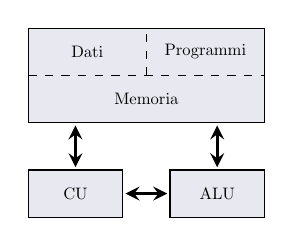
\begin{tikzpicture}[scale=0.6, every node/.style={scale=0.6}]
    \filldraw[fill=MidnightBlue!10!white] (0,0) rectangle ++(5,2);
    \draw[dashed] (0,1) -- (5,1) (2.5,1) -- (2.5,2);
    \filldraw[fill=MidnightBlue!10!white] (0,-2) rectangle ++(2,1);
    \filldraw[fill=MidnightBlue!10!white] (3,-2) rectangle ++(2,1);
    \path (2.5,0.5) node {Memoria}
          (1.25,1.5) node {Dati}
          (3.75,1.5) node {Programmi}
          (1,-1.5) node {CU}
          (4,-1.5) node {ALU};
    \draw[stealth-stealth,very thick,shorten >=1pt,shorten <=1pt] (2,-1.5) -- (3,-1.5);
    \draw[stealth-stealth,very thick,shorten >=1pt,shorten <=1pt] (1,-1) -- (1,0);
    \draw[stealth-stealth,very thick,shorten >=1pt,shorten <=1pt] (4,-1) -- (4,0);
  \end{tikzpicture}\end{center}
  \vfill
  \begin{itemize}
    \item Memoria unica per dati e programmi
    \vfill
    \item CU (Control Unit): assegna e gestisce risorse
    \vfill
    \item ALU (Arithmetic Logic Unit): compie operazioni
    \vfill
    \item ALU + CU = CPU (Central Processing Unit)
  \end{itemize}
  \vfill
\end{frame}

\begin{frame}{CPU}
  \vfill
  \begin{itemize}
    \item La CPU esegue istruzioni \alert{semplici}
    \vfill
    \item Istruzione tipo:
    \begin{itemize}
      \item che operazione fare
      \item indirizzi di memoria degli operandi
      \item indirizzi di memoria dei risultati
    \end{itemize}
    \vfill
    \item Le istruzioni sono codificate come numeri binari
    \vfill
    \item Le istruzioni eseguibili dipendono dal tipo di CPU
  \end{itemize}
  \vfill
\end{frame}

\begin{frame}{Assembly}
  \vfill
  \begin{itemize}
    \item I linguaggi \alert{assembly} hanno una corrispondenza 1-ad-1
    con le istruzioni della macchina
    \vfill
    \item Le istruzioni vengono ``tradotte'' da numeri binari a parole comprensibili
    ad un essere umano
    \vfill
    \item Un programma in assembly è una lista di istruzioni che la CPU eseguirà
    nell'ordine in cui appaiono
    \vfill
    \item CPU diverse hanno linguaggi assembly diversi
  \end{itemize}
  \vfill
\end{frame}

\begin{frame}{Assembly}
  \vfill
  \begin{center}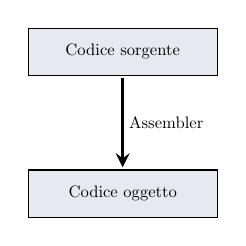
\begin{tikzpicture}[scale=0.6, every node/.style={scale=0.6}]
    \filldraw[fill=MidnightBlue!10!white] (0,0) rectangle ++(4,1);
    \filldraw[fill=MidnightBlue!10!white] (0,-3) rectangle ++(4,1);
    \path (2,0.5) node {Codice sorgente}
          (2,-2.5) node {Codice oggetto};
    \draw[-stealth,very thick,shorten >=1pt,shorten <=1pt] (2,0) -- node[right] {Assembler} (2,-2);
  \end{tikzpicture}\end{center}
  \vfill
  \begin{itemize}
    \item Il \alert{codice sorgente} è un file contenente testo
    \vfill
    \item Il \alert{codice oggetto} è un file contenente istruzioni binarie
    \vfill
    \item Un programma detto \alert{assembler} converte il codice sorgente in codice
    oggetto, eseguibile dalla CPU
  \end{itemize}
  \vfill
\end{frame}

\begin{frame}{Linguaggi di programmazione}
  \vfill
  \begin{itemize}
    \item Un \alert{linguaggio} di programmazione è un linguaggio \alert{formale}
    con il quale scrivere istruzioni
    \begin{itemize}
      \item distinzione tra istruzioni valide/invalide
      \item le istruzioni controllano la CPU
    \end{itemize}
    \vfill
    \item Distinzione di \alert{livello}
    \begin{itemize}
      \item basso livello: \alert{1-ad-1} con istruzioni della CPU
      \item alto livello: linguaggi \alert{astratti}
    \end{itemize}
    \vfill
    \item Un \alert{paradigma di programmazione} è uno stile secondo il quale
    viene scritto il codice sorgente
    \vfill
    \item Ciascun linguaggio accetta uno o più paradigmi
  \end{itemize}
  \vfill
\end{frame}

\begin{frame}{Linguaggi compilati}
  \vfill
  \begin{center}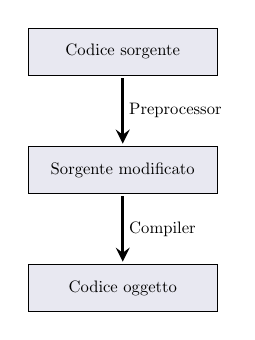
\begin{tikzpicture}[scale=0.6, every node/.style={scale=0.6}]
    \filldraw[fill=MidnightBlue!10!white] (0,0) rectangle ++(4,1);
    \filldraw[fill=MidnightBlue!10!white] (0,-2.5) rectangle ++(4,1);
    \filldraw[fill=MidnightBlue!10!white] (0,-5) rectangle ++(4,1);
    \path (2,0.5) node {Codice sorgente}
          (2,-2) node {Sorgente modificato}
          (2,-4.5) node {Codice oggetto};
    \draw[-stealth,very thick,shorten >=1pt,shorten <=1pt] (2,0) -- node[right] {Preprocessor} (2,-1.5);
    \draw[-stealth,very thick,shorten >=1pt,shorten <=1pt] (2,-2.5) -- node[right] {Compiler} (2,-4);
  \end{tikzpicture}\end{center}
  \vfill
  \begin{itemize}
    \item Il codice sorgente viene scritto per intero \vfill
    \item Il \alert{preprocessor} modifica al sorgente (facoltativo) \vfill
    \item Il \alert{compiler} crea un file oggetto dal sorgente
  \end{itemize}
  \vfill
\end{frame}

\begin{frame}{Linguaggi interpretati}
  \vfill
  \begin{center}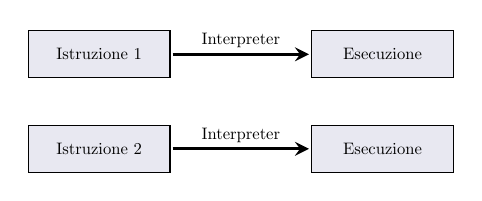
\begin{tikzpicture}[scale=0.6, every node/.style={scale=0.6}]
    \filldraw[fill=MidnightBlue!10!white] (0,0) rectangle ++(3,1);
    \filldraw[fill=MidnightBlue!10!white] (6,0) rectangle ++(3,1);
    \path (1.5,0.5) node {Istruzione 1};
    \path (7.5,0.5) node {Esecuzione};
    \draw[-stealth,very thick,shorten >=1pt,shorten <=1pt] (3,0.5) -- node[above] {Interpreter} (6,0.5);
    \begin{scope}[shift={(0,-2)}]
      \filldraw[fill=MidnightBlue!10!white] (0,0) rectangle ++(3,1);
      \filldraw[fill=MidnightBlue!10!white] (6,0) rectangle ++(3,1);
      \path (1.5,0.5) node {Istruzione 2};
      \path (7.5,0.5) node {Esecuzione};
      \draw[-stealth,very thick,shorten >=1pt,shorten <=1pt] (3,0.5) -- node[above] {Interpreter} (6,0.5);
    \end{scope}
  \end{tikzpicture}\end{center}
  \vfill
  \begin{itemize}
    \item Ciascuna istruzione viene compilata singolarmente
    \vfill
    \item Esecuzione di programm incompleti
    \vfill
    \item Molto più lenti dei linguaggi compilati
  \end{itemize}
  \vfill
\end{frame}

\begin{frame}{Paradigmi}
  \vfill
  \begin{itemize}
    \item Programmazione imperativa
    \begin{itemize}
      \item lista di \alert{comandi} eseguiti in un certo ordine
    \end{itemize}
    \vfill
    \item Programmazione dichiarativa
    \begin{itemize}
      \item lista di \alert{relazioni} tra enti
    \end{itemize}
    \vfill
    \item Programmazione ad oggetti
    \begin{itemize}
      \item lista di \alert{oggetti} e di \alert{interazioni} tra essi
    \end{itemize}
  \end{itemize}
  \vfill
\end{frame}

\begin{frame}{Programmazione imperativa}
  \vfill
  \begin{itemize}
    \item Scrittura di un \alert{algoritmo} per risolvere un problema
    \vfill
    \item Esempio: cambiare la batteria di un telecomando
    \begin{itemize}
      \item aprire il vano batterie
      \item rimuovere la vecchia batteria
      \item gettare la vecchia batteria
      \item inserire la nuova batteria
      \item chiudere il vano batterie
    \end{itemize}
    \vfill
    \item L'ordine delle istruzioni è determinante
  \end{itemize}
  \vfill
\end{frame}

\begin{frame}{Flowcharts}
  \vfill
  \begin{itemize}
    \item Per rappresentare un algoritmo si utilizzano i \alert{flowcharts} o \alert{diagrammi di flusso}
    \vfill
    \item Un flowchart è costituito da
    \begin{itemize}
      \item celle contenenti istruzioni
      \item frecce che guidano il \alert{flusso di controllo}
    \end{itemize}
    \vfill
    \item I flowcharts sono un linguaggio di programmazione
    \vfill
    \item Creare flowcharts aiuta nella stesura di un algoritmo
  \end{itemize}
  \vfill
\end{frame}

\begin{frame}{Flowcharts}
  \vfill
  \begin{center}\begin{tikzpicture}[node distance=15mm]
  \node[begin] (start) at (0,0) {\textbf{BEGIN}};
  \draw[arrow] (start) to ++(0,-1);
  \node[begin] (end) at (4,-0.75) {\textbf{END}};
  \draw[arrow] (4,0.25) to (end);
  \end{tikzpicture}\end{center}
  \vfill
  \begin{itemize}
    \item Istruzioni di inizio e fine diagramma
    \vfill
    \item Uno ed un solo \alert{BEGIN} per diagramma
    \vfill
    \item A volte ammessi più \alert{END} in un singolo diagramma
  \end{itemize}
\end{frame}

\begin{frame}{Flowcharts}
  \vfill
  \begin{center}\begin{tikzpicture}[node distance=15mm]
  \node[operation] (op) at (0,0) {operazione};
  \draw[arrow] (op) to ++(0,-1);
  \draw[arrow] (0,1) to (op);
  \end{tikzpicture}\end{center}
  \vfill
  \begin{itemize}
    \item Istruzione di processo
    \vfill
    \item Viene eseguita l'operazione indicata nella casella
  \end{itemize}
\end{frame}

\begin{frame}{Flowcharts}
  \vfill
  \begin{center}\begin{tikzpicture}[node distance=15mm]
    \node[begin] (start) {\textbf{BEGIN}};
    \node[below of=start,operation](init){\(a = 1+1\)};
    \node[below of=init,begin](end){\textbf{END}};

    \draw[arrow] (start) to (init);
    \draw[arrow] (init) to (end);
  \end{tikzpicture}\end{center}
  \vfill
  \begin{itemize}
    \item Il programma calcola 1+1 \vfill
    \item Il risultato viene messo nella \alert{variabile} \(a\)
  \end{itemize}
\end{frame}

\begin{frame}{Flowcharts}
  \vfill
  \begin{center}\begin{tikzpicture}[node distance=15mm]
  \node[input] (in) at (0,0) {\textbf{READ} \(x\)};
  \draw[arrow] (in) to ++(0,-1);
  \draw[arrow] (0,1) to (in);
  \node[output] (out) at (4,0) {\textbf{WRITE} \(x\)};
  \draw[arrow] (out) to ++(0,-1);
  \draw[arrow] (4,1) to (out);
  \end{tikzpicture}\end{center}
  \vfill
  \begin{itemize}
    \item Istruzioni di lettura/scrittura
    \vfill
    \item Lettura: un valore inserito dall'\alert{utente} viene memorizzato nella
    variabile \(x\)
    \vfill
    \item Scrittura: il valore corrente della variabile \(x\) viene comunicato all'\alert{utente}
  \end{itemize}
\end{frame}

\begin{frame}{Flowcharts}
  \vfill
  \begin{center}\begin{tikzpicture}[node distance=15mm]
    \node[begin] (start) {\textbf{BEGIN}};
    \node[below of=start,input](in){\textbf{READ} \(a\)};
    \node[below of=in,operation](op){\(a = a+1\)};
    \node[below of=op,output](out){\textbf{WRITE} \(a\)};
    \node[below of=out,begin](end){\textbf{END}};

    \draw[arrow] (start) to (in);
    \draw[arrow] (in) to (op);
    \draw[arrow] (op) to (out);
    \draw[arrow] (out) to (end);
  \end{tikzpicture}\end{center}
  \vfill
\end{frame}

\begin{frame}{Flowcharts}
  \vfill
  \begin{center}\begin{tikzpicture}[node distance=15mm]
  \node[decision] (op) at (0,0) {condizione};
  \draw[arrow] (op) to node[above]{no} ++(3,0);
  \draw[arrow] (op) to node[above]{sì} ++(-3,0);
  \draw[arrow] (0,2) to (op);
  \end{tikzpicture}\end{center}
  \vfill
  \begin{itemize}
    \item Istruzione condizionale
    \vfill
    \item Il flusso del grafico cambia direzione a seconda che la condizione
    sia vera oppure falsa
  \end{itemize}
\end{frame}

\begin{frame}{Flowcharts}
  \vfill
  \begin{center}\begin{tikzpicture}[node distance=15mm]
  \node[connection] (cn) at (0,0) {};
  \draw[arrow] (cn) to ++(0,-1);
  \draw[arrow] (-1,0) to (cn);
  \draw[arrow] (1,0) to (cn);
  \end{tikzpicture}\end{center}
  \vfill
  \begin{itemize}
    \item Connettore
    \vfill
    \item Permette di rincongiungere due rami separati
  \end{itemize}
\end{frame}

\begin{frame}{Flowcharts}
  \vfill
  \begin{center}\begin{tikzpicture}[scale=0.9, every node/.style={scale=0.9},node distance=15mm]
    \node[begin] (start) {\textbf{BEGIN}};
    \node[below of=start,input](in){\textbf{READ} \(a\)};
    \node[below of=in,decision](dec){\(a \in \mathbb{P}\)};
    \node[below right = 8mm and 10mm of dec,output](pari){\textbf{WRITE} ``pari''};
    \node[below left = 8mm and 10mm of dec,output](dispari){\textbf{WRITE} ``dispari''};
    \node[below = 20mm of dec,connection](conn){};
    \node[below of=conn,begin](end){\textbf{END}};

    \draw[arrow] (start) to (in);
    \draw[arrow] (in) to (dec);
    \draw[arrow] (dec) -| node[above] {no} (dispari);
    \draw[arrow] (dec) -| node[above] {sì} (pari);
    \draw[arrow] (dispari) |- (conn);
    \draw[arrow] (pari) |- (conn);
    \draw[arrow] (conn) to (end);
  \end{tikzpicture}\end{center}
  \vfill
\end{frame}

\begin{frame}{Flowcharts}
  \vfill
  \begin{itemize}
    \item Le regole elencate danno origine alla programmazione imperativa in senso lato
    \vfill
    \item Le frecce possono ``risalire'' il diagramma
    \begin{itemize}
      \item istruzioni \alert{goto}: ritorno ad un punto precedente
    \end{itemize}
    \vfill
    \item Questo rende più difficile:
    \begin{itemize}
      \item studio formale del programma
      \item apportare modifiche al codice
      \item comprensione del programma da parte di terzi
    \end{itemize}
  \end{itemize}
\end{frame}

\begin{frame}{Flowcharts}
  \vfill
  \begin{itemize}
    \item La programmazione \alert{strutturata} vieta i goto
    \vfill
    \item Le frecce non possono risalire il diagramma
    \vfill
    \item Viene aggiunto un nuovo simbolo
    \vfill
    \item Teorema di Böhm-Jacopini
    \begin{itemize}
      \item \alert{equivalenza} tra imperativa e strutturata
    \end{itemize}
  \end{itemize}
\end{frame}

\begin{frame}{Flowcharts}
  \vfill
  \begin{center}\begin{tikzpicture}[node distance=15mm]
  \node[loop] (op) at (0,0) {condizione};
  \draw[arrow] (op) to node[left]{no} ++(0,-1);
  \draw[arrow] (op) to node[above]{sì} ++(2.5,0) to ++(0,.5);
  \draw[arrow] (0,1) to (op);
  \end{tikzpicture}\end{center}
  \vfill
  \begin{itemize}
    \item Istruzione di loop
    \vfill
    \item Concettualmente identica all'istruzione condizionale, ma uno (ed uno solo)
    dei due flussi può risalire
    \vfill
    \item Permette di ripetere una serie di istruzioni
  \end{itemize}
\end{frame}

\begin{frame}{Flowcharts}
  \vfill
  \begin{center}\begin{tikzpicture}[scale=0.6, every node/.style={scale=0.6},node distance=13mm]
    \node[begin] (start) {\textbf{BEGIN}};
    \node[below of=start,input] (read) {\textbf{READ} \(a\)};
    \node[below of=read,connection] (conn) {};
    \node[below of=conn,output] (write) {\textbf{WRITE} \(a\)};
    \node[below of=write,operation](decr){\(a = a-1\)};
    \node[below of=decr,loop](loop){\(a \neq 0\)};
    \node[below = 6mm of loop,begin](end){\textbf{END}};

    \draw[arrow] (start) to (read);
    \draw[arrow] (read) to (conn);
    \draw[arrow] (conn) to (write);
    \draw[arrow] (write) to (decr);
    \draw[arrow] (decr) to (loop);
    \draw[arrow] (loop) to node[anchor=east]{no} (end);
    \draw[arrow] (loop) to node[anchor=south]{sì} ++(20mm,0) |- (conn);
  \end{tikzpicture}\end{center}
  \vfill
\end{frame}

\begin{frame}{Flowcharts}
  \vfill
  \begin{center}\begin{tikzpicture}[scale=0.6, every node/.style={scale=0.6},node distance=13mm]
    \node[begin] (start) {\textbf{BEGIN}};
    \node[below of=start,operation](init){\(s = 0\)};
    \node[below of=init,input] (read) {\textbf{READ} \(a\)};
    \node[below of=read,connection] (conn) {};
    \node[below of=conn,operation](add){\(s = s+a\)};
    \node[below of=add,operation](decr){\(a = a-1\)};
    \node[below of=decr,loop](loop){\(a \neq 0\)};
    \node[below = 6mm of loop,output] (write) {\textbf{WRITE} \(s\)};
    \node[below of=write,begin](end){\textbf{END}};

    \draw[arrow] (start) to (init);
    \draw[arrow] (init) to (read);
    \draw[arrow] (read) to (conn);
    \draw[arrow] (conn) to (add);
    \draw[arrow] (add) to (decr);
    \draw[arrow] (decr) to (loop);
    \draw[arrow] (loop) to node[anchor=east]{no} (write);
    \draw[arrow] (loop) to node[anchor=south]{sì} ++(20mm,0) |- (conn);
  \draw[arrow] (write) to (end);
  \end{tikzpicture}\end{center}
  \vfill
\end{frame}
